\subsubsection{Spoof Access Point}
\label{sec:spoofap}
This is not necessarily an attack in itself, but a means of relying on social engineering to gain connections to perform attacks on. A soft access point is a rogue access point that has been established on a wireless adaptor, without the need for a router. Leaving this open, and performing in an area with a high footfall, or cafe area, for example, will allow the attacker to gain connections, monitor traffic, and perform various man-in-the-middle attacks, including ones mentioned in section \ref{mitm-sec}. It can also be paired with other attacks, as demonstrated in section \ref{ddos-atk}.

\begin{figure}[h!]
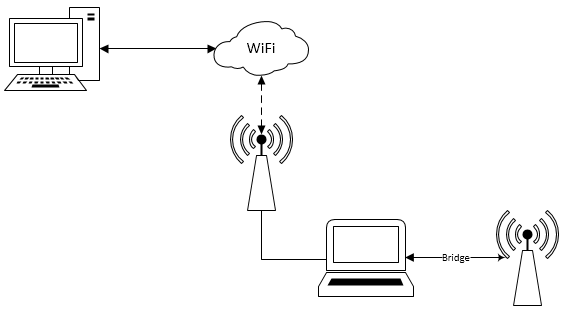
\includegraphics[width=\linewidth]{research/figures/spoofap.png}
\caption{Soft access point bridges traffic to real access point.}
\end{figure}

\subsubsection*{Performing the Attack}
As this is more of a gateway attack, not a lot can be gained from doing it alone. The airbase-ng tool proved the best way to create a fake access point, taking the wireless interface and either start or stop as parameters, as shown in figure \ref{ssid-demo-sec}. In this demonstration the laptop is running BackTrack and is using the Alfa wireless adaptor. The image below shows the creation of an access point and a station connecting to it.

\begin{figure}[h!]
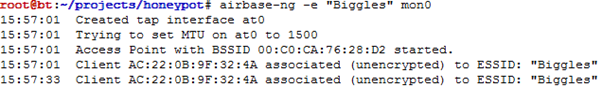
\includegraphics[width=\linewidth]{research/attackvectors/figures/spoofap1.png}
\caption{Soft access point created with the SSID “Biggles”.}
\label{ssid-demo-sec}
\end{figure}